%%=========================================
%\chapter{About \ce{CdZnTe}}
%%=========================================
%\ce{CdZnTe} is a compound semiconductor material composed of elements belonging to the II and VI groups of the periodic table of chemical elements.

%\section{Crystal structure}
%The crystal structure of \acl{czt} consist of two face centred cubic lattices with one shifted from the other by $\frac{1}{4}$ of the distance along the (111) direction. One lattice is occupied by \ce{Te} and a fraction $x$ of the other lattice is occupied by \ce{Zn} while the remaining fraction of the other lattice is occupied by \ce{Cd}.
%%=========================================
%\section{Band structure}
%Figure~\ref{fig:} clearly demonstrates that the band gap of \ac{mct} can be tuned to .. \mycomment{???}
%%=========================================
\chapter{Experimental Details}\label{ch:exp-details}
In this chapter, a description of the substrates, the pre-growth surface preparation methods, and the experimental equipment is presented.

\section{Epitaxy}

Epitaxy refers to the growth of a crystalline layer with a well-defined orientation determined by the crystal structure of a substrate. One of the epitaxial growth techniques is \acf{lpe} where a layer is grown from a supersaturated liquid solution on a substrate. The process starts with heating the solution, followed by a period where impurities are baked out. After this, the temperature is lowered to equilibrium, and then the growth is achieved by reducing the temperature so that the material deposit on the substrate. Another epitaxial growth technique is \acf{mbe} where a source material is heated to produce an evaporated beam of particles. Then the constituent elements of the wanted material are transported through vacuum from the sources to the substrate where it condenses.

%%=========================================
\section{CdZnTe Substrates}
%\todo{CZT advantages: excellent lattice match, CT good passivation. Disadvantage: brittle brakes easily, expensive.}

\Acl{czt} substrates with $y=\SI{0.04}{}$ are mainly \ce{CdTe} with a small fraction of the \ce{Cd} atoms replaced by \ce{Zn} atoms in order to match the substrate lattice constant to that of \acl{mct} (\SI{6.46}{}-\SI{6.48}{\angstrom}). \Ac{czt} has a zincblende structure with two interpenetrating face-centered cubic lattices offset by $\parentheses{\frac{1}{4},\frac{1}{4},\frac{1}{4}}a$, where $a$ is the lattice constant in the primitive cell. Cadmium or zinc atoms form one of the sublattices while tellurium atoms form the other, as seen in Fig.~\ref{fig:zincblende-structure}.

\begin{figure}[htbp]
    \centering
    \mySubfigure{0.302\linewidth}{zinc-blende.png}[fig:zincblende-structure]
    \hfill
    \mySubfigure{0.679\linewidth}{zinc-blende_faces.png}[fig:zincblende-face]
    \caption[Crystal structure of \ac{czt}.]{Illustration of \subref{fig:zincblende-structure} the zincblende crystal structure of \ac{czt} and \subref{fig:zincblende-face} the difference between the two faces of a (111)-oriented \ac{czt} substrate (or the (111)-oriented steps in a (211)-oriented substrate). The plane will have top and bottom surfaces that are slightly different: the A face is terminated by triply bonded \ce{Cd} (or \ce{Zn}) or singly bonded \ce{Te}, while the B face is terminated by triply bonded \ce{Te} or singly bonded \ce{Cd} (or \ce{Zn}). \ce{Cd} (or \ce{Zn}) atoms form the white sublattice and \ce{Te} atoms form the black sublattice \citep[Adapted from][]{sivananthan1986relation}.}
    \label{fig:zincblende}
\end{figure}

The orientation of the substrate is given by the surface crystallographic plane, and for \ac{czt} substrates the crystal is cut to give surface plane (111) for \ac{lpe} growth and (211) for \ac{mbe} growth. The (211)-oriented substrate consists of steps that are (111)-oriented. A substrate cut along these planes will have top and bottom surfaces that are slightly different: one surface will be terminated by triply bonded \ce{Cd} (or \ce{Zn}) or singly bonded \ce{Te}, and is called the \emph{A} face, while the other side of the substrate will be terminated by triply bonded \ce{Te} or singly bonded \ce{Cd} (or \ce{Zn}), and is called the \emph{B} face \citep{sivananthan1986relation}, see Fig.~\ref{fig:zincblende-face}. \Ac{mct} films are always grown on the B face of the substrate since it is less sensitive to misorientation \citep{parker1988terracing, edwall1984liquid}.%$y$ is the fraction of cadmium that is substituted with zinc and $1-y$ is the fraction of cadmium \citep{zha2005atomic}. \Ac{czt}

In this study, two (111)B-oriented substrates from different manufacturers and one (211)B-oriented substrate have been studied. Substrate A is a $\SI{30}{\milli\metre}\times\SI{30}{\milli\metre}$ state-of-the-art (111)B-oriented \ac{czt} substrate from the Japanese firm JX Nippon Mining \& Metals Corporation (vendor A). The $y$-value in substrate A is \SIrange{2.8}{3.6}{\percent}. Substrate A was compared to substrate B -- a $\SI{30}{\milli\metre}\times\SI{30}{\milli\metre}$ (111)B-oriented \ac{czt} substrate -- from an alternative source (vendor B). Substrate B has \SI{\sim 4}{\percent} \ce{Zn} and \SI{\sim96}{\percent} \ce{Cd}. Substrate C is a $15\times$\SI{15}{\milli\metre^2} state-of-the-art (211)B-oriented \ac{czt} substrate also from vendor A. The $y$-value in substrate C is \SIrange{2.6}{3.4}{\percent}. % vendor B: Klamnik, Keystone

Images of the substrates can be seen in Fig.~\ref{fig:substrateABC}. Relative terms, such as \emph{upper}, \emph{lower}, \emph{left}, \emph{right}, and \emph{centre}, are used to describe the locations on the substrate surfaces throughout the thesis. These relative terms are related to the orientation depicted in Fig.~\ref{fig:substrateABC}. When coordinates are given, they are measured from the lower left corner of the substrate surfaces. %\todo{Nevne koordinatsystem her? Eller droppe koordinater og heller bruke lower left corner, etc.?}

The substrates were characterised as-received and after surface pre-growth preparation. The latter was either polishing and etching or just etching if the substrate was already polished by the vendor. Then \iac{mct} layer was grown on each substrate and characterised with emphasis on the correlation between defects in the \ac{mct} layer and particles, impurities, defects and roughness of the substrates.

Unfortunately, after being characterised both as-received and after polish and etch, substrate B broke in two pieces when mounting for the final \ac{ftir} mapping before \ac{mct} growth. One piece shattered further when it fell on the floor, as seen in Fig.~\ref{fig:subBb_photo_pieces}. These substrates are brittle, and all the handling of the substrate through two rounds of characterisation with various techniques had made it even more so. A new $\SI{30}{\milli\metre}\times\SI{30}{\milli\metre}$ (111)B-oriented \ac{czt} substrate from vendor B, substrate B2, was polished and characterised before growing \iac{mct} layer on it.
%Substrate B was unfortunately shattered during preparation for \ac{ftir} even though the preparation procedure was followed as normal, see Fig.~\ref{fig:subB_om_6x_pieces}. It could be the additional handling, i.e. due to the extensive characterisation, that caused it to be more fragile. Substrate B was already studied as-received and with surface pre-growth preparation (except for \ac{ftir}). The next step was to grow \iac{mct} film on it. To be able to fulfil the process, an additional substrate from vendor B was studied (substrate B2). Substrate B2 is a $\SI{30}{\milli\metre}\times\SI{30}{\milli\metre}$  (111)B-oriented \ac{czt} substrate and has \SI{\sim 4}{\percent} \ce{ZnTe} and \SI{\sim96}{\percent} \ce{CdTe}. Due to lack of time, substrate B2 was only studied after surface pre-growth preparation before \iac{mct} film was grown on it.

\begin{figure}[htbp]
    \centering
    \mySubfigure{0.48\linewidth}{subAa_om_6x.png}[fig:subAa_photo]
    \hfill
    \mySubfigure{0.48\linewidth}{subBb_om_6x.png}[fig:subBb_photo]
    \par\bigskip
    \mySubfigure{0.48\linewidth}{subB2b_om_6x.png}[fig:subB2b_photo]
    \hfill
    \mySubfigure{0.48\linewidth}{subCa_om_6x.png}[fig:subCa_photo]
    \par\bigskip
    \mySubfigure{0.48\linewidth}{subBb_om_pieces.png}[fig:subBb_photo_pieces]
    \caption[Optical microscopy images of the substrates.]{Optical microscopy images of the substrates. \subref{fig:subAa_photo} Substrate A -- as-received, $\SI{30}{\milli\metre}\times\SI{30}{\milli\metre}$, (111)B-oriented from vendor A; \subref{fig:subBb_photo} substrate B -- after polish and etch, $\SI{30}{\milli\metre}\times\SI{30}{\milli\metre}$, (111)B-oriented from vendor B; \subref{fig:subB2b_photo} substrate B2 -- after polish and etch, $\SI{30}{\milli\metre}\times\SI{30}{\milli\metre}$, (111)B-oriented from vendor B; \subref{fig:subCa_photo} Substrate C -- as-received, $\SI{15}{\milli\metre}\times\SI{15}{\milli\metre}$, (211)B-oriented from vendor A; and \subref{fig:subBb_photo_pieces} substrate B after it shattered during mounting for \ac{ftir}.}
    % \todo{Optical microscopy images of the substrates. a) Substrate A: Asreceived, 30x30mm2 from vendor A, b) .. and 15x15mm2 substrates}
    \label{fig:substrateABC}
\end{figure}

Vendor A sells both (111)B-oriented substrates for \ac{lpe} growth and (211)B-oriented substrates for \ac{mbe} growth. The (211)B substrates are cut at an angle of \SI{19}{\degree} with the (111) planes. This gives a surface with (111)-oriented atomic steps, and the resulting step-flow growth improves the crystallinity of the \ac{mbe} film because atoms land on the surface and diffuse to a step edge before they nucleate, and hence, reduce the change of dislocations. 

High-quality substrate surfaces are crucial for growth of high-quality films. After cutting, the substrates must be polished to obtain the necessary smooth and planar surface. Finally, an etch is needed to remove polishing products that have been trapped in the substrate during polishing. In \ac{lpe} growth, the outermost layers of the substrate are initially melting in the liquid growth material before the temperature falls and the film starts to grow on the surface. Therefore, some surface defects can be less important while others remain and affect the grown film.

%Substrates from two vendors were compared: One state-of-the-art \ac{lpe} substrate (substrate A) and one state-of-the-art \ac{mbe} substrate (substrate C) from the Japanese manufacturer JX Nippon Mining \& Metals Corporation (vendor A), and one \ac{lpe} substrate (substrate B) from an alternative source (vendor B). Substrate A and B was polished by the vendor and needed only a short etch before growth, while substrate B required both polishing and etching before growth.
%
%% The substrates:
% --- A:  with lot number BZ1503 and wafer number ID7.1, Zn concentration Specification 0.025+-0.05 Measurements 0.028-0.036
% --- B:  with number C-3895-23
% --- B*: with number C-4040-8
% --- C:  with lot number BZ1204 and wafer number ID10.4, Zn concentration Specification 0.035+-0.01 Measurements 0.026-0.034

%%=========================================
\section{As-Received}
The substrates were removed from the box they came in and directly mounted on carbon tape on a \ac{sem} holder before \ac{sem} was performed. To ensure that the removal process would be as easy as possible, the carbon tape was made almost non-sticky by touching the tape multiple times with a cleanroom glove. A magnetic plate was attached underneath the \ac{sem} holder with double-sided tape when \ac{afm} was performed. 

To remove the substrate from the \ac{sem} holder, the holder with the substrate on top was placed in a beaker, and acetone was poured into the beaker up to right below the backside of the substrate. The acetone dissolved the carbon tape so that it was possible to get a scalpel under the substrate and push the substrate off. %\todo{Mention problems with tape removal.}

%%=========================================
\section{Pre-Growth Surface Preparation}
It is important to have the surface as smooth and planar as possible and without any particles to grow high-quality \ac{mct} film. Hence, substrate preparation is an important part before the deposition of a crystalline layer takes place. The three substrates were prepared in the following way: Substrate A and C needed only an etch before growth since they were already sufficiently polished by the vendor. Substrate B and B2 needed a final polish as part of their pre-growth preparation in addition to an etch since they only had been through a coarse polish by the vendor. The surface preparation procedures will be described in more detail in the following paragraphs.

\subsection{Etching of Substrate A}\label{sec:subA_etch}

After the characterisation of the as-received substrate A was completed, the substrate went through a standard \ac{lpe} \ce{Br}:methanol preparation etch procedure. First, the substrate was cleaned using a two-solvent method. The two-solvent cleaning procedure consists of placing the substrate for \SIrange{2}{3}{\minute} in each of four containers: two with boiling acetone, one with boiling methanol, and one with methanol at room temperature. Before further preparation, the substrate was blown dry with gaseous nitrogen. Then, the substrate was etched in an etch consisting of \SI{0.25}{\milli\litre} bromine and \SI{40}{\milli\litre} methanol for \SI{30}{\second} while stirring every \SIrange{1}{2}{\second}. Finally, the substrate was rinsed with methanol to remove any etch residues. This \ce{Br}:methanol etch procedure was repeated before \ac{lpe} growth with an etch time of \SI{50}{\second} to remove possible contaminants from the characterisation of the etched substrate. %When the substrate is lifted from one container, it is rinsed with \todo{skriv ned det steget her.}

\subsection{Polishing and Etching of Substrate B}

After the characterisation of the as-received substrates B and B2 was completed, the substrates were cleaned using soap, rinsed with purified water, and then blown dry with gaseous nitrogen. This is the standard \ac{lpe} preparation procedure before polishing and etching take place, but due to the exposure during characterisation and the potential residue of carbon tape underneath substrate B, it had to go through an additional cleaning procedure with a two-solvent method, as explained in Section~\ref{sec:subA_etch}.%\todo{mention that this was not enough, maybe?}

%The as-received substrate A was etched \todo{with a Bromine-based etch}. The substrate was already polished when received from the vendor.
%
% Sprutet på såpe over hele substratet. Skylt av med renvann. Blåst tørr med nitrogen. 
% Vanligvis kun såpe, men nå kokende aceton og metanol pga. det kan sitte igjen litt karbonteip fra holderen. Lagt i kokende aceton i noen få minutter, skylt med aceton fra spruteflaske for å få vekk det som har løsnet og ikke få det med videre, lagt i kokende aceton igjen noen få minutter, sprutet med aceton deretter metanol før lagt i kokende metanol noen få minutter, spylt med metanol, og til sist lagt i romtemperert metanol i noen minutter. Blåst tørr med nitrogengass.
% Montert på glassplate med Crytalbond. Varmer opp Crystalbond slik at det smelter og renner under substratet. Avkjøles. Sitter fast.
% Festet opp ned i jig med vakuum på glassplata. Roterende skive med hard poleringspad pusser substratet plant, 50 um. Bytter til myk poleringspad og pusser substratet jevnt, 30 um, 111 minutter. Drypper på poleringsvæske jevnt og trutt (med pumpe). Kjell Ove har også på "lubricat" når skiva begynner å gå litt sakte (alkohol og ++).
% Skyller med renvann. Blåser tørr med nitrogen.
% Fjernet poleringssøl som har samlet seg langs med endekantene ved bruk av q-tips. Drar de langs med kanten. Bruker en bred q-tip til å fjerne det som ligger på glassplaten. Det legger seg mye poleringssøl langs endekantene. Sannsynligvis oppå substratet også.
% Spruter på såpe over hele substratet. Har såpe på en bomullsdott og drar denne over substratet forsiktig. Tar ny bomullsdott og bløter og drar over.
% Skyller med aceton. Blåser tørr med nitrogen.
% Varmer opp glassplata på varmeplate (150 grader celsius) slik at Crystalbond smelter, og det er mulig å skyve av substratet med hjelp av en spatel. Og over i en hvit rund silplate med stang til å duppe opp og ned i begerglass.
% Samme kokende aceton og kokende metanol prosedyre som over.
% Ligger i romtemperert metanol over natta (fra 20.03.17 14.00 til 21.03.17 12.00).

The as-received substrates B and B2 were polished with alumina powders with an abrasive size of \SI{50}{\nano\metre} using a Struers LaboPol-5 polishing jig. First, the substrate was planarised by removing an average of \SI{80}{\micro\metre} of material from the surface of the substrate with a hard polishing pad for \SI{200}{\minute}. Then a smoother finish was achieved by removing another \SI{30}{\micro\metre} of material from the surface using a soft polishing pad for \SI{111}{\minute}. The soft polishing pad conforms to local topology variations on the nanoscopic scale, and thus, makes the surface smooth, while hard pads do not \citep{lee2000nanotopography}. The polishing slurry consisted of \SI{50}{\nano\metre} colloidal alumina particles and soap dissolved in methanol. The use of soap as a lubricant is helpful in prolonging the life of the polishing jig.

During polishing the substrate was attached to a plate using Crystalbond mounting compound. The Crystalbond was melted underneath the substrate to form an adhesive bond between the substrate and the mounting plate when solidifying. After the polishing process was completed, the mounting plate was heated to melt the Crystalbond so that the substrate could be pushed off. Then the remaining Crystalbond was dissolved and removed through the same two-solvent cleaning procedure as before polishing. The cleaned substrate was soaked in a beaker with methanol at room temperature overnight before it was etched with a \ce{Br}:methanol etch the following day, as described for substrate A in Section~\ref{sec:subA_etch}, and quickly inserted into the \ac{sem}.

\subsection{Etching of Substrate C}
%The as-received substrate C was etched \todo{with a Bromine-based etch}. The substrate was already polished when received from the vendor.

After the characterisation of the as-received substrate C was completed, the substrate went through a standard \ac{mbe} \ce{Br}:methanol preparation etch procedure. First, the substrate was cleaned with methanol and acetone: A thin layer of methanol was left on the surface for \SIrange{2}{3}{\second} before it was blown dry with gaseous nitrogen, and the equivalent was repeated with acetone and finally with methanol for the second time. Then, the substrate was etched in \SI{1}{\percent} \ce{Br}:methanol for \SI{2}{\minute} while gently stirring every \SI{30}{\second}. Finally, the substrate was rinsed by soaking the substrate in multiple beakers filled with methanol.

%\todo{The current state-of-the-art \ac{mbe} preparation etch for (211)B \ac{czt} consists of an organic solvent surface clean, \ce{Br}:methanol etch, methanol rinse, and deionised water rinse \citep{benson1996situ}.} \todo{The substrates were methanol soaked for \SI{5}{\minute}. Then they were bromine methanol (\SI{0.3}{\percent}) etched for \SI{2}{\minute}. Lastly they were rinsed with distilled deionised water and blown dry with nitrogen.}
%\todo{The polished samples were chemically etched with \ce{Br}-\ce{MeOH} using different concentrations to determine the optimal concentration for high quality surface finish. Concentrations of bromine between \SI{1}{} and \SI{4}{\percent} were investigated and each sample was etched for a duration of \SI{30}{\second}. \ce{Br}-methanol is one of the most common etching solutions for \ce{CdZnTe} \citep{li2006thermal}.}}


%%=========================================
\section{Equipment}

%A Wild Heerbrugg M650 optical microscope was used to capture  

A Leica DM RXA2 optical microscope was used to capture dark field optical microscopy images. These images were used to locate irregularities in the substrate surface, known as morphological defects, characterise the surface topography, and count the density of large particles and defects (\SI{>0.5}{\micro\metre}).

Transmission \ac{ir} microscopy was performed using the Leica DM RXA2 optical microscope with transmitted illumination from a halogen light lamp at \SI{3450}{\kelvin} under the stage and a BU238M \ac{ir} camera from Toshiba Teli for image recording. The band gap in \ac{czt} is \SI{1.6}{\electronvolt}. Hence, photons with energy greater than the band gap, i.e. wavelengths smaller than \SI{775}{\nano\metre}, are not transmitted through the substrate. The \ac{ir} camera can detect photons with wavelengths between \SI{200}{\nano\metre} and \SI{1125}{\nano\metre}. This results in the detection of photons with wavelengths between \SI{775}{\nano\metre} and \SI{1125}{\nano\metre}, as seen in Fig.~\ref{fig:ir-range}. The \ac{ir} transmission images were used to study tellurium precipitates inside the substrate. %\todo{Hvorfor har Espen skrevet 900? Se Matlab-fil.}
% Plate med hull slik at urenheter på og i glasset unngås. 7.5cm x 7.5cm

\begin{figure}[htbp]
    \centering
    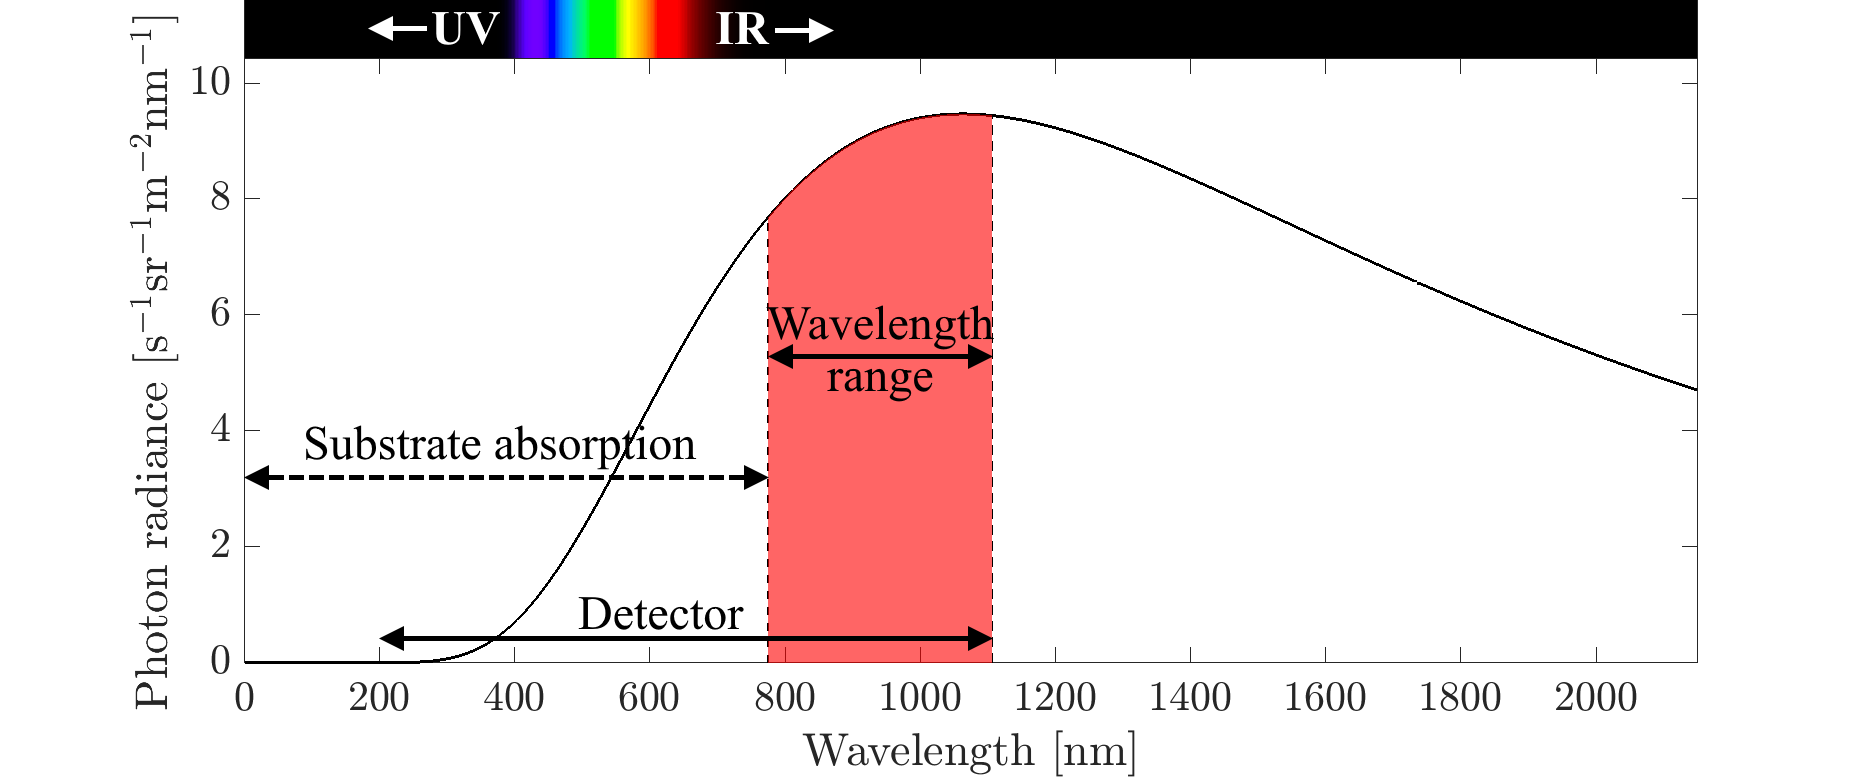
\includegraphics[width=1.0\linewidth,,trim={1.6cm 0cm 1.6cm 0cm},clip]{blackbody_photon_radiance.png}
    \caption[Graph showing the wavelength range of the near-\ac{ir} transmission microscopy setup.]{The wavelength range of the near-\ac{ir} transmission microscopy setup used in this study. The black curve is the number of photons emitted per unit wavelength per second per steradian from one square meter of a perfect black-body at a temperature of \SI{3450}{\kelvin} given by Planck's law of black-body radiation, see Eq.~\eqref{eq:planck-law}. The red area represents the photons that are transmitted through the sample and detected by the \ac{ir} camera, i.e. have an energy smaller than the bandgap of \ac{czt} (\SI{>775}{\nano\metre}),  and has an energy within the detector range of the \ac{ir}-camera (\SIrange{200}{1125}{\nano\metre}). The coloured bar above the graph illustrates at which wavelengths ultraviolet (UV), visible, and infrared (IR) radiation are found.}
    \label{fig:ir-range}
\end{figure}

%Bruker XFlash 5010 semiconductor silicon drift detector for energy dispersive spectrometers
%A Hitachi Model SU6600 Variable pressure Schottky field emission gun scanning electron microscope with a Bruker XFlash 5010 detector for the energy-dispersive X-ray spectrometer was used to find and identify defects, damage, and particles on the substrate surfaces. The \ac{sem} is capable of much higher magnifications and has a greater resolving power than the optical microscope. Hence, it can see much smaller objects in finer detail. A quantitative determination of the chemical composition of different areas and features were obtained using the Bruker Quantax Microanalysis System software.
A Hitachi Model SU6600 Variable pressure Schottky field emission gun scanning electron microscope was used to find defects, damage, and particles on the substrate surfaces. The \ac{sem} is capable of much higher magnifications and has a greater resolving power than the optical microscope. Hence, it can see much smaller features in finer detail. The \ac{sem} is equipped with a Bruker XFlash 5010 detector for the energy-dispersive X-ray spectrometer. \Ac{eds} was used to identify the composition of defects, damage, and particles on the substrate surfaces. A quantitative determination of the chemical composition of different areas and features was obtained using the Bruker Quantax Microanalysis System software.

\Ac{xps} measurements were carried out with a SPECS system equipped with an \ce{Al}/\ce{Mg} twin anode XR50 X-ray source and a Riber MAC2 analyser. The \ce{Mg} anode was operated at \SI{300}{\watt} and the X-ray beam was incident at \SI{45}{\degree} with the sample normal, while emitted photoelectrons were collected in the analyser at \SI{30}{\degree}. The data was retrieved from the Riber MAC2 control unit by Cameca's Kernel 3 software, and surface composition was determined with standard methods described by \citet{moulder2000handbook} using intensity peak areas, obtained using Systat Software's PeakFit program, and elemental sensitivity factors measured experimentally on the \ac{xps} equipment at \ac{ffi} by \citet{hirsch1999x-ray}.% Or Cameca with Riber EA 150

%The \ac{xps} equipment is situated in a vacuum chamber that is attached to the \ac{mbe} machine. Samples are mounted on molybdenum blocks before they go into this machine. However, as the \ac{xps} X-ray beam diameter is as large as \SI{1}{\centi\metre}, and spectra both in the middle and along the sides of the substrates were going to be acquired, the material for the holder surrounding the substrate had to be chosen so that it did not have peaks overlapping with the elements of interest in this study. After careful considerations it was decided to make the holder from titanium, whose binding energies do not overlap with those of either \ce{Cd}, \ce{Te}, \ce{Zn}, \ce{Hg}, \ce{Al}, \ce{Si}, \ce{Cl}, \ce{S}, \ce{P}, \ce{Fe}, \ce{Br}, \ce{Cu}, \ce{O}, or \ce{C}, which are either observed in our acquired \ac{eds} spectra or found by \citet{benson2015as-received}.
%The substrate was placed in a titanium stand and secured by two titanium plates in the corners before being mounted onto a molybdenum block, and then inserted into the introduction chamber of the vacuum system before being transferred to the surface analysis chamber. The \ac{xps} data were acquired with \ce{Mg} K$\alpha$ x-ray radiation from a non-monochromatic source having an energy of \SI{1253.6}{\electronvolt}.

%With the large beam size we could only hope to see traces of impurity elements over a large area, but not locate them to specific particles or areas. Also, photoelectrons are only emitted if emitted from an atom within approximately \SI{80}{\angstrom} from the surface, so the technique can only tell us about the outermost layer of the sample. Unfortunately, something was broken on the old analyser, resulting in low signal intensity and no detection of impurities or small concentrations of elements. The ever-present oxide and carbon overlayers further decreased any small signals. Therefore, the \ac{xps} only gave information about the following elements: \ce{Te}, \ce{Cd}, \ce{O} and \ce{C}.
%Due to low count rates it was not possible to get enough statistics to detect surface impurities. Due to the low quality of the results, only substrate A was characterised using this technique.

Topographic mapping of the surfaces was performed with a Park Systems XE-100 atomic force microscope. The \ac{afm} images were recorded in non-contact mode using a Nanosensors PPP-NCHR probe with an aluminium coating on the detector side. The images were obtained using a scan rate of \SI{0.2}{\hertz} and a scan size of \SI{5}{\micro\metre}. The \ac{afm} is capable of much higher depth and height resolution than the other techniques, and hence, it can be used to obtain greater detail of surface irregularities like scratches and voids.

A Perkin Elmer Spectrum GX \ac{ftir} system was used to obtain transmission spectra of the substrates. The spectra present the \ac{ir} transmittance of the substrates in the wavenumber range of \SIrange{370}{5000}{\centi\metre^{-1}}. They were used to get information about the density and size of tellurium precipitates, the free carrier concentration, and the resistivity of the substrates. % to see how much light that is transmitted through the material at the different \ac{ir} wavelengths

%%=========================================